\ESKDappendix{рекомендуемое}{Терминология относительных измерений}\label{app_relative_relativity}
Относительно координат некоторых векторов, являющихся в большинстве своем некоторыми кинематическими величинами, в тексте документа можно встретить указания на то, что они получены (или отсчитаны) <<\dots относитель\-но такой-то системы координат\dots>> и при этом <<\dots выражены относительно такой-то системы координат\dots>>.
Это приложение разъясняет смысл данных фраз нижеследующим простым примером.

Рассмотрим рисунок~\ref{img:tree_cart_and_bird}.
На нем изображены стоящий неподвижно куст, тележка, катящаяся со скоростью $v=1\text{ м/с}$, облако, движущееся со скоростью $u=3\text{ м/с}$, и жестко связанные с ними правосторонние системы координат $Ox_0y_0z_0$, $Ox_1y_1z_1$ и $Ox_2y_2z_2$.
Опишем скорость движения облака вектором~$V$.
В~зависимости от своего физического смысла он будет иметь разные координаты.
Наглядно это демонстрирует таблица~\ref{table_values_of_v}.

\begin{figure}[h!]
	\centering
	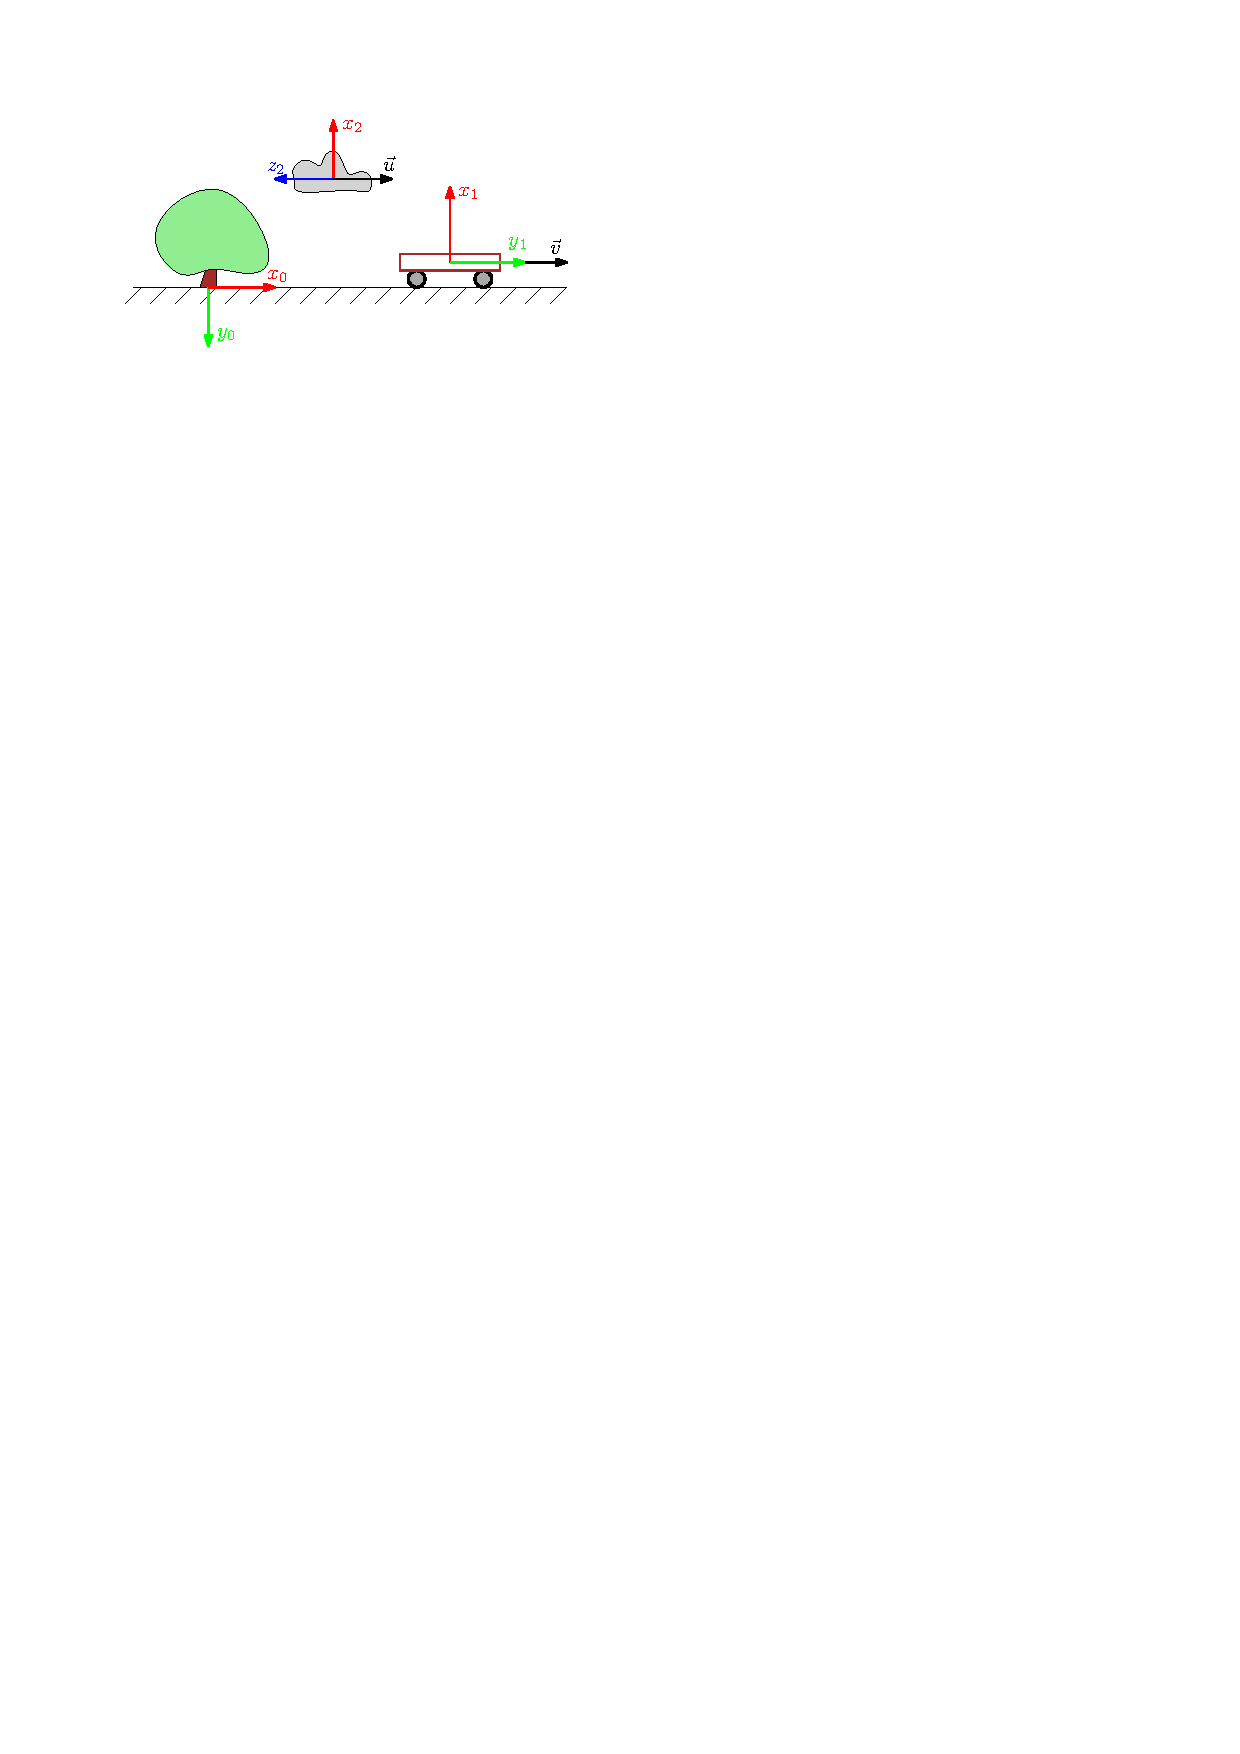
\includegraphics[width=0.9\textwidth]{tree_cart_and_bird.pdf}
	\caption{Воображаемая ситуация из пояснительного примера.}
	\label{img:tree_cart_and_bird}
\end{figure}

\begin{table}[h!]
	\caption{Координаты вектора $V$ в зависимости от его физического смысла.}
	\begin{center}
		\begin{tabular}{|m{13cm}|m{3cm}|}
			\hline
			\multicolumn{1}{|c|}{Смысл вектора $V$} & \makebox[3cm]{Значение $V^T$}\\
			\hline
			Скорость $Ox_2y_2z_2$ относительно $Ox_0y_0z_0$, выраженная относительно $Ox_0y_0z_0$ & $$\begin{bmatrix}3 & 0 & 0\end{bmatrix}$$\\
			\hline
			Скорость $Ox_2y_2z_2$ относительно $Ox_0y_0z_0$, выраженная относительно $Ox_1y_1z_1$ & $$\begin{bmatrix}0 & 3 & 0\end{bmatrix}$$\\
			\hline
			Скорость $Ox_2y_2z_2$ относительно $Ox_0y_0z_0$, выраженная относительно $Ox_2y_2z_2$ & $$\begin{bmatrix}0 & 0 & -3\end{bmatrix}$$\\
			\hline
			Скорость $Ox_2y_2z_2$ относительно $Ox_1y_1z_1$, выраженная относительно $Ox_0y_0z_0$ & $$\begin{bmatrix}2 & 0 & 0\end{bmatrix}$$\\
			\hline
			Скорость $Ox_2y_2z_2$ относительно $Ox_1y_1z_1$, выраженная относительно $Ox_1y_1z_1$ & $$\begin{bmatrix}0 & 2 & 0\end{bmatrix}$$\\
			\hline
			Скорость $Ox_2y_2z_2$ относительно $Ox_1y_1z_1$, выраженная относительно $Ox_2y_2z_2$ & $$\begin{bmatrix}0 & 0 & -2\end{bmatrix}$$\\
			\hline
		\end{tabular}
	\end{center}
	\label{table_values_of_v}
\end{table}

